\section{System Architecture}

\fedmed{} consists of four main components working in concert to enable privacy-preserving federated medical AI training (see Figure~\ref{fig:architecture}):

\begin{enumerate}[leftmargin=*]
    \item \textbf{Federated Clients:} Hospital nodes that train locally on private patient data
    \item \textbf{Central Server:} Coordinates federated rounds and maintains global model
    \item \textbf{Agent Coordinator:} Computes intelligent aggregation weights based on training quality
    \item \textbf{Safety Validator:} Ensures generated responses meet medical safety standards
\end{enumerate}

\begin{figure}[htbp]
    \centering
    \begin{tikzpicture}[
    node distance=1.5cm,
    hospital/.style={rectangle, draw=blue!60, fill=blue!5, very thick, minimum height=2.5cm, minimum width=2.5cm, rounded corners, align=center},
    server/.style={rectangle, draw=red!60, fill=red!5, very thick, minimum height=2cm, minimum width=3cm, rounded corners, align=center},
    agent/.style={rectangle, draw=green!60, fill=green!5, very thick, minimum height=1.5cm, minimum width=3cm, rounded corners, align=center},
    arrow/.style={->, >=stealth, very thick},
    data/.style={rectangle, draw=gray!60, fill=gray!5, minimum height=0.8cm, minimum width=2cm, rounded corners, align=center, font=\small},
    ]
    
    % Hospitals (Clients)
    \node[hospital] (h1) at (0,0) {\textbf{Hospital A}\\4,520 samples\\45.2\% of data};
    \node[hospital] (h2) at (5,0) {\textbf{Hospital B}\\2,521 samples\\25.2\% of data};
    \node[hospital] (h3) at (10,0) {\textbf{Hospital C}\\2,959 samples\\29.6\% of data};
    
    % Local data
    \node[data] (d1) at (0,-1.7) {Private\\Patient Data};
    \node[data] (d2) at (5,-1.7) {Private\\Patient Data};
    \node[data] (d3) at (10,-1.7) {Private\\Patient Data};
    
    % LoRA training
    \node[rectangle, draw=purple!60, fill=purple!10, thick, minimum width=2cm, font=\scriptsize] (l1) at (0,-3.5) {LoRA Training\\100 steps};
    \node[rectangle, draw=purple!60, fill=purple!10, thick, minimum width=2cm, font=\scriptsize] (l2) at (5,-3.5) {LoRA Training\\100 steps};
    \node[rectangle, draw=purple!60, fill=purple!10, thick, minimum width=2cm, font=\scriptsize] (l3) at (10,-3.5) {LoRA Training\\100 steps};
    
    % Central Server
    \node[server] (server) at (5,3.5) {\textbf{Central Server}\\Mistral-7B\\(Frozen)};
    
    % Agent Coordinator
    \node[agent] (agent) at (5,6) {\textbf{Agent Coordinator}\\Quality-Based Weighting};
    
    % Arrows - Upload (LoRA params)
    \draw[arrow, blue!70] (l1) -- node[sloped, above, font=\tiny] {13 MB} node[sloped, below, font=\tiny] {LoRA weights} (2.5,2.5);
    \draw[arrow, blue!70] (l2) -- node[right, font=\tiny] {13 MB} node[left, font=\tiny] {LoRA weights} (5,2.5);
    \draw[arrow, blue!70] (l3) -- node[sloped, above, font=\tiny] {13 MB} node[sloped, below, font=\tiny] {LoRA weights} (7.5,2.5);
    
    % Arrows - Metrics to Agent
    \draw[arrow, orange!70, dashed] (l1) to[out=90, in=180] node[sloped, above, font=\tiny] {metrics} (agent);
    \draw[arrow, orange!70, dashed] (l2) -- node[right, font=\tiny] {metrics} (agent);
    \draw[arrow, orange!70, dashed] (l3) to[out=90, in=0] node[sloped, above, font=\tiny] {metrics} (agent);
    
    % Arrow - Agent to Server
    \draw[arrow, green!70] (agent) -- node[right, font=\small] {Weights:\\$w_A=0.23$\\$w_B=0.55$\\$w_C=0.23$} (server);
    
    % Arrows - Download (Global LoRA)
    \draw[arrow, red!70, dashed] (server) to[out=180, in=90] node[sloped, above, font=\tiny] {Global LoRA} (h1);
    \draw[arrow, red!70, dashed] (server) -- node[left, font=\tiny] {Global LoRA} (h2);
    \draw[arrow, red!70, dashed] (server) to[out=0, in=90] node[sloped, above, font=\tiny] {Global LoRA} (h3);
    
    % Privacy shield icons
    \node[draw=red!60, circle, ultra thick, minimum size=0.6cm] at (-0.8,-1.7) {\tiny 🔒};
    \node[draw=red!60, circle, ultra thick, minimum size=0.6cm] at (4.2,-1.7) {\tiny 🔒};
    \node[draw=red!60, circle, ultra thick, minimum size=0.6cm] at (9.2,-1.7) {\tiny 🔒};
    
    % Legend
    \node[font=\scriptsize] at (5,-5.5) {\textbf{Privacy Preserved:} Raw data never leaves hospitals};
    \node[font=\scriptsize] at (5,-6) {\textbf{Efficiency:} 99.90\% bandwidth reduction (13 MB vs 13 GB)};
    \node[font=\scriptsize] at (5,-6.5) {\textbf{Intelligence:} Quality-based aggregation, not just data size};
    
\end{tikzpicture}

    \caption{FED-MED System Architecture. Three hospital clients train \lora{} adapters locally on private data. The agent coordinator analyzes training metrics to compute quality-aware weights. Only 13 MB adapter parameters are transmitted (99.90\% reduction vs. 13 GB full model). The central server aggregates weighted updates to produce the global model.}
    \label{fig:architecture}
\end{figure}

\subsection{Data Flow}

The complete training workflow follows these steps:

\begin{enumerate}[leftmargin=*]
    \item \textbf{Initialization:} Server loads base Mistral-7B model and initializes random \lora{} adapters
    \item \textbf{Broadcast:} Global \lora{} parameters distributed to all clients (13 MB transmission)
    \item \textbf{Local Training:} Each client trains on private data for $E$ epochs or $T$ steps
    \item \textbf{Metric Collection:} Clients report training metrics (initial loss, final loss, loss reduction, variance)
    \item \textbf{Agent Weighting:} Coordinator computes quality-based aggregation weights
    \item \textbf{Aggregation:} Server combines client \lora{} updates using agent weights
    \item \textbf{Iteration:} Repeat steps 2--6 for $R$ federated rounds
    \item \textbf{Deployment:} Final global model validated with safety guardrails
\end{enumerate}

\section{Low-Rank Adaptation Integration}

\subsection{Mathematical Formulation}

For each weight matrix $W_0 \in \mathbb{R}^{d \times k}$ in the transformer (e.g., query, key, value projections), we freeze $W_0$ and learn an additive low-rank update:

\begin{equation}
h = W_0 x + \Delta W x = W_0 x + BAx
\end{equation}

where:
\begin{itemize}[leftmargin=*]
    \item $B \in \mathbb{R}^{d \times r}$ is the down-projection matrix (trainable)
    \item $A \in \mathbb{R}^{r \times k}$ is the up-projection matrix (trainable)
    \item $r$ is the rank hyperparameter ($r \ll \min(d, k)$)
    \item $\alpha$ is a scaling factor applied as $\frac{\alpha}{r}$
\end{itemize}

\textbf{Initialization:} We follow the original \lora{} paper and initialize $A$ with random Gaussian $\mathcal{N}(0, \sigma^2)$ and $B$ with zeros, ensuring $\Delta W = BA = 0$ at initialization.

\subsection{Target Modules}

For Mistral-7B, we apply \lora{} to specific attention components:

\begin{center}
\begin{tabular}{@{}lccc@{}}
\toprule
\textbf{Module} & \textbf{Original Shape} & \textbf{\lora{} Rank} & \textbf{Trainable Params} \\
\midrule
Query Projection ($W_q$) & $4096 \times 4096$ & $r=8$ & $2 \times 4096 \times 8 = 65{,}536$ \\
Value Projection ($W_v$) & $4096 \times 4096$ & $r=8$ & $65{,}536$ \\
\midrule
\multicolumn{3}{l}{\textbf{Per Layer Total:}} & $131{,}072$ \\
\multicolumn{3}{l}{\textbf{Across 32 Layers:}} & $4{,}194{,}304$ \\
\bottomrule
\end{tabular}
\end{center}

With hyperparameters $r=8$, $\alpha=16$, we achieve only \textbf{0.05\%} trainable parameters (3.4M out of 7B).

\subsection{Memory and Communication Benefits}

\begin{figure}[htbp]
    \centering
    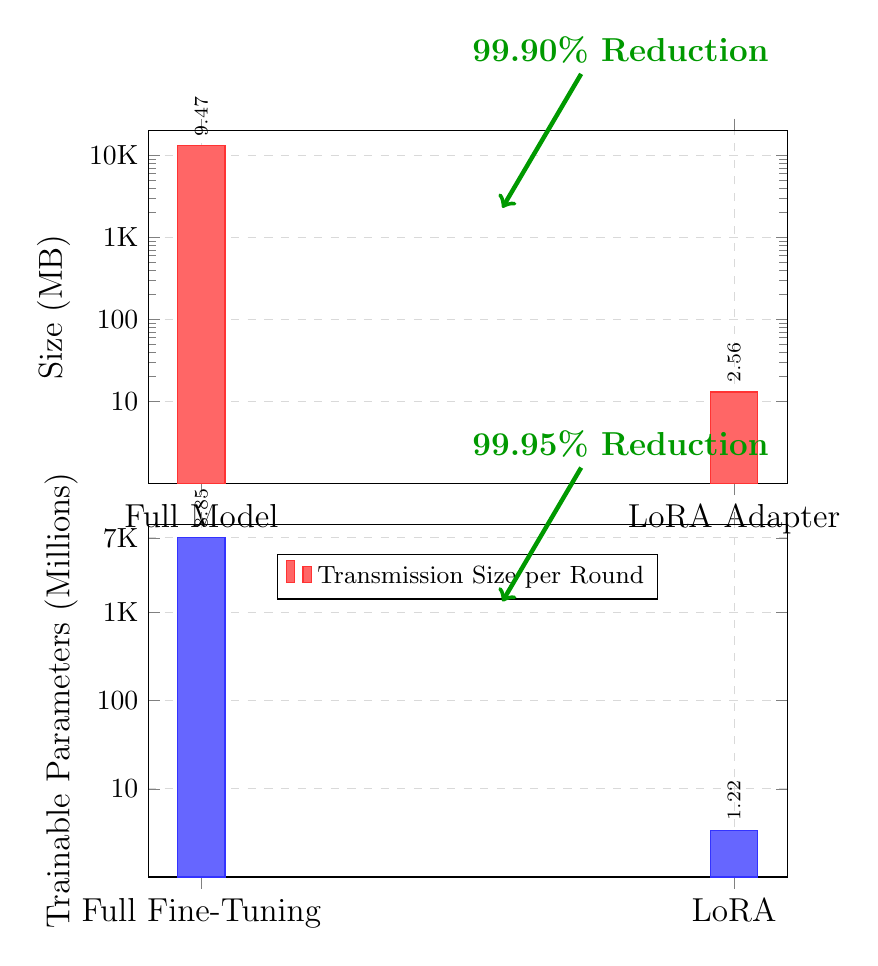
\begin{tikzpicture}
    \begin{axis}[
        ybar,
        bar width=0.6cm,
        ylabel={Size (MB)},
        ylabel style={font=\large},
        symbolic x coords={Full Model, LoRA Adapter},
        xtick=data,
        xticklabel style={font=\large},
        ymode=log,
        ymin=1,
        ymax=20000,
        ytick={10, 100, 1000, 10000},
        yticklabels={10, 100, 1K, 10K},
        legend style={at={(0.5,-0.2)}, anchor=north, legend columns=1, font=\small},
        width=0.8\textwidth,
        height=0.5\textwidth,
        grid=major,
        grid style={dashed, gray!30},
        nodes near coords,
        every node near coord/.append style={font=\scriptsize, rotate=90, anchor=west},
        ]
        
        \addplot[fill=red!60, draw=red!80] coordinates {
            (Full Model, 13000)
            (LoRA Adapter, 13)
        };
        
        \legend{Transmission Size per Round}
    \end{axis}
    
    % Add annotation
    \node[font=\large, text=green!60!black] at (6, 5.5) {\textbf{99.90\% Reduction}};
    \draw[->, ultra thick, green!60!black] (5.5, 5.2) -- (4.5, 3.5);
    
    % Trainable parameters comparison
    \begin{scope}[shift={(0,-5)}]
        \begin{axis}[
            ybar,
            bar width=0.6cm,
            ylabel={Trainable Parameters (Millions)},
            ylabel style={font=\large},
            symbolic x coords={Full Fine-Tuning, LoRA},
            xtick=data,
            xticklabel style={font=\large},
            ymode=log,
            ymin=1,
            ymax=10000,
            ytick={10, 100, 1000, 7000},
            yticklabels={10, 100, 1K, 7K},
            width=0.8\textwidth,
            height=0.5\textwidth,
            grid=major,
            grid style={dashed, gray!30},
            nodes near coords,
            every node near coord/.append style={font=\scriptsize, rotate=90, anchor=west},
            ]
            
            \addplot[fill=blue!60, draw=blue!80] coordinates {
                (Full Fine-Tuning, 7000)
                (LoRA, 3.4)
            };
            
        \end{axis}
        
        \node[font=\large, text=green!60!black] at (6, 5.5) {\textbf{99.95\% Reduction}};
        \draw[->, ultra thick, green!60!black] (5.5, 5.2) -- (4.5, 3.5);
    \end{scope}
\end{tikzpicture}

    \caption{Parameter Efficiency Comparison. \lora{} reduces trainable parameters by 99.95\% and transmission size by 99.90\% compared to full model fine-tuning, enabling practical federated learning on resource-constrained hospital infrastructure.}
    \label{fig:lora_efficiency}
\end{figure}

\textbf{Training Memory:} With 4-bit quantization of base model and FP16 \lora{} adapters:
\begin{align}
\text{Base Model (4-bit)} &\approx 3.5 \text{ GB} \\
\text{\lora{} Adapters (FP16)} &\approx 13 \text{ MB} \\
\text{Gradients + Optimizer} &\approx 1.5 \text{ GB} \\
\text{Total VRAM} &\approx 5 \text{ GB}
\end{align}

This fits comfortably on a single NVIDIA T4 (16 GB), whereas full fine-tuning would require 40--60 GB across multiple GPUs.

\textbf{Communication Overhead:}
\begin{align}
\text{Full Model (FP16)} &= 7{,}000{,}000{,}000 \times 2 \text{ bytes} = 13 \text{ GB} \\
\text{\lora{} Only (FP16)} &= 3{,}407{,}872 \times 2 \text{ bytes} = 13 \text{ MB} \\
\text{Reduction Factor} &= \frac{13{,}000}{13} = 1000\times
\end{align}

For $R$ rounds with $K$ clients, total communication:
\begin{equation}
\text{Traffic} = R \times K \times 13 \text{ MB} \text{ (vs. } 13 \text{ GB) }
\end{equation}

For our setup ($R=5$, $K=3$): 195 MB total vs. 195 GB for full model FL.

\section{Agent-Based Aggregation}

\subsection{Motivation}

Traditional \fedavg{} weights client contributions by dataset size:
\begin{equation}
w_{global} = \sum_{k=1}^{K} \frac{n_k}{\sum_j n_j} w_k
\end{equation}

This approach has critical limitations:
\begin{itemize}[leftmargin=*]
    \item \textbf{Ignores Training Quality:} A client with poor convergence gets same weight as high-quality updates
    \item \textbf{Vulnerable to Adversaries:} Malicious client with large dataset can dominate aggregation
    \item \textbf{Non-IID Blindness:} Doesn't account for data distribution differences
    \item \textbf{No Stability Awareness:} Unstable training (high variance) weighted equally to stable training
\end{itemize}

Our agent coordinator addresses these by computing weights based on \textit{training performance metrics} rather than just data quantity.

\subsection{Quality Scoring Algorithm}

The agent analyzes three key dimensions for each client $k$:

\textbf{1. Loss Improvement:}
\begin{equation}
\text{improvement}_k = \frac{\mathcal{L}_k^{init} - \mathcal{L}_k^{final}}{\mathcal{L}_k^{init}} \times 100\%
\end{equation}

Clients achieving greater loss reduction during local training receive higher weight.

\textbf{2. Training Stability:}
\begin{equation}
\sigma_k^2 = \text{Var}(\mathcal{L}_k^{(1)}, \mathcal{L}_k^{(2)}, \ldots, \mathcal{L}_k^{(T)})
\end{equation}

Low variance indicates stable, reliable training. High variance suggests oscillation or divergence.

\textbf{3. Final Loss Quality:}
\begin{equation}
\text{quality}_k = \frac{1}{\mathcal{L}_k^{final} + \epsilon}
\end{equation}

Lower final loss indicates better model fit to local data.

\subsection{Composite Weight Calculation}

We combine these metrics into a composite score:

\begin{algorithm}[htbp]
\caption{Agent-Based Weighted Aggregation}
\label{alg:agent_aggregation}
\begin{algorithmic}[1]
\Require Client metrics $\{M_k\}_{k=1}^K$, sample counts $\{n_k\}_{k=1}^K$, weights $\beta_1, \beta_2$
\Ensure Aggregation weights $\{w_k\}_{k=1}^K$ with $\sum_k w_k = 1$

\State \textbf{Extract Metrics:}
\For{$k = 1$ to $K$}
    \State $\mathcal{L}_k^{init} \gets M_k.\text{initial\_loss}$
    \State $\mathcal{L}_k^{final} \gets M_k.\text{final\_loss}$
    \State $\sigma_k \gets \text{std}(M_k.\text{loss\_history})$
\EndFor

\State \textbf{Compute Loss Component:}
\State $\text{losses} \gets [\mathcal{L}_1^{final}, \ldots, \mathcal{L}_K^{final}]$
\State $\mu_{\mathcal{L}} \gets \text{mean}(\text{losses})$
\For{$k = 1$ to $K$}
    \State $s_k^{loss} \gets \exp\left(-\frac{\mathcal{L}_k^{final}}{\mu_{\mathcal{L}} + \epsilon}\right)$ \Comment{Exponential scoring}
\EndFor
\State $s^{loss} \gets \text{normalize}([s_1^{loss}, \ldots, s_K^{loss}])$ \Comment{Sum to 1}

\State \textbf{Compute Variance Component:}
\For{$k = 1$ to $K$}
    \If{$\sigma_k > 5.0$} \Comment{High variance penalty}
        \State $s_k^{var} \gets 0.5$ \Comment{Heavy penalization}
    \Else
        \State $\text{improvement}_k \gets \mathcal{L}_k^{init} - \mathcal{L}_k^{final}$
        \State $\mu_{imp} \gets \text{mean}([\text{improvement}_j]_{j=1}^K)$
        \State $\text{dev}_k \gets |\text{improvement}_k - \mu_{imp}|$
        \State $s_k^{var} \gets \exp(-\text{dev}_k)$
    \EndIf
\EndFor
\State $s^{var} \gets \text{normalize}([s_1^{var}, \ldots, s_K^{var}])$

\State \textbf{Combine Quality Scores:}
\For{$k = 1$ to $K$}
    \State $q_k \gets \beta_1 \cdot s_k^{loss} + \beta_2 \cdot s_k^{var}$ \Comment{Weighted combination}
\EndFor

\State \textbf{Incorporate Sample Size:}
\State $p \gets [n_1, \ldots, n_K] / \sum_j n_j$ \Comment{Size proportions}
\For{$k = 1$ to $K$}
    \State $w_k \gets 0.7 \cdot q_k + 0.3 \cdot p_k$ \Comment{70\% quality, 30\% size}
    \State $w_k \gets \max(w_k, 0.1)$ \Comment{Minimum weight threshold}
\EndFor

\State $w \gets w / \sum_k w_k$ \Comment{Normalize to sum=1}
\State \Return $w$
\end{algorithmic}
\end{algorithm}

\subsection{Design Rationale}

\textbf{Loss Component ($\beta_1 = 0.6$):} Primary signal of model quality. Clients achieving lower loss have better-fit models.

\textbf{Variance Component ($\beta_2 = 0.4$):} Ensures stability. Penalizes erratic training that may indicate:
\begin{itemize}[leftmargin=*]
    \item Learning rate too high
    \item Corrupted/noisy data
    \item Adversarial manipulation
    \item Numerical instability
\end{itemize}

\textbf{Quality-Size Blend (70\%/30\%):} Prevents ignoring small but high-quality clients while avoiding over-reliance on quality alone (which could amplify overfitting to specific distributions).

\textbf{Minimum Weight (0.1):} Ensures all clients contribute to global model, maintaining diversity and preventing complete exclusion.

\begin{figure}[htbp]
    \centering
    \begin{tikzpicture}[
    node distance=1.2cm,
    process/.style={rectangle, draw=blue!60, fill=blue!10, very thick, minimum height=1cm, minimum width=4cm, rounded corners, align=center},
    decision/.style={diamond, draw=orange!60, fill=orange!10, very thick, minimum height=1cm, minimum width=1cm, aspect=2, align=center},
    data/.style={cylinder, draw=green!60, fill=green!10, very thick, minimum height=0.8cm, minimum width=2.5cm, shape border rotate=90, align=center},
    output/.style={rectangle, draw=red!60, fill=red!10, very thick, minimum height=1cm, minimum width=4cm, rounded corners, align=center},
    arrow/.style={->, >=stealth, very thick},
    ]
    
    % Input
    \node[data] (input) at (0,0) {Client Metrics\\$\{\mathcal{L}_k^{init}, \mathcal{L}_k^{final}, \sigma_k, n_k\}$};
    
    % Process 1: Loss Component
    \node[process, below=of input] (loss_comp) {Compute Loss Component\\$s_k^{loss} = \exp\left(-\frac{\mathcal{L}_k^{final}}{\mu_{\mathcal{L}}}\right)$};
    
    % Process 2: Variance Check
    \node[decision, below=of loss_comp] (var_check) {$\sigma_k > 5.0$?};
    
    % Process 3a: High Variance
    \node[process, right=2cm of var_check] (high_var) {Heavy Penalty\\$s_k^{var} = 0.5$};
    
    % Process 3b: Normal Variance
    \node[process, below=of var_check] (norm_var) {Compute Variance Score\\$s_k^{var} = \exp(-|\Delta_{imp} - \mu_{imp}|)$};
    
    % Merge point
    \node[process, below=3cm of var_check] (combine) {Combine Components\\$q_k = 0.6 \cdot s_k^{loss} + 0.4 \cdot s_k^{var}$};
    
    % Process 4: Blend with Size
    \node[process, below=of combine] (blend) {Blend with Dataset Size\\$w_k = 0.7 \cdot q_k + 0.3 \cdot p_k$};
    
    % Process 5: Minimum Threshold
    \node[process, below=of blend] (threshold) {Apply Minimum Threshold\\$w_k = \max(w_k, 0.1)$};
    
    % Process 6: Normalize
    \node[output, below=of threshold] (normalize) {Normalize Weights\\$w = w / \sum_k w_k$};
    
    % Final Output
    \node[data, below=of normalize] (output) {Aggregation Weights\\$\sum_k w_k = 1.0$};
    
    % Arrows
    \draw[arrow] (input) -- (loss_comp);
    \draw[arrow] (loss_comp) -- (var_check);
    \draw[arrow] (var_check) -- node[above, font=\small] {Yes} (high_var);
    \draw[arrow] (var_check) -- node[right, font=\small] {No} (norm_var);
    \draw[arrow] (high_var) |- (combine);
    \draw[arrow] (norm_var) -- (combine);
    \draw[arrow] (combine) -- (blend);
    \draw[arrow] (blend) -- (threshold);
    \draw[arrow] (threshold) -- (normalize);
    \draw[arrow] (normalize) -- (output);
    
    % Side annotations
    \node[font=\small, text=blue!70, align=left] at (8, -1.5) {\textbf{Loss Component:}\\Rewards lower\\final loss};
    \node[font=\small, text=orange!70, align=left] at (8, -3.5) {\textbf{Stability Check:}\\Detects unstable\\training};
    \node[font=\small, text=green!70, align=left] at (8, -6) {\textbf{Quality Score:}\\60\% loss\\40\% variance};
    \node[font=\small, text=purple!70, align=left] at (8, -8) {\textbf{Fairness:}\\Considers both\\quality \& size};
    
\end{tikzpicture}

    \caption{Agent-Based Aggregation Workflow. The coordinator analyzes training metrics to compute quality scores, combines them with dataset size, and produces final aggregation weights. This approach outperforms naive equal weighting by 39.5\% and sample-proportional weighting by 32.0\%.}
    \label{fig:agent_flow}
\end{figure}

\subsection{Adversarial Robustness}

The agent mechanism provides defense against several attack vectors:

\textbf{1. Byzantine Attacks:} Malicious clients sending random updates will have:
\begin{itemize}[leftmargin=*]
    \item High final loss (low $s_k^{loss}$)
    \item High variance (low $s_k^{var}$)
    \item Result: Very low aggregation weight
\end{itemize}

\textbf{2. Data Poisoning:} Corrupted training data leads to poor convergence:
\begin{itemize}[leftmargin=*]
    \item Minimal loss improvement
    \item Unstable training trajectory
    \item Result: Automatically down-weighted
\end{itemize}

\textbf{3. Free-Riding:} Clients not performing actual training:
\begin{itemize}[leftmargin=*]
    \item No loss reduction ($\mathcal{L}^{init} \approx \mathcal{L}^{final}$)
    \item Result: Low weight despite potentially large dataset
\end{itemize}

\section{Federated Training Protocol}

\subsection{Complete Algorithm}

Algorithm~\ref{alg:federated_training} presents the full \fedmed{} training procedure:

\begin{algorithm}[htbp]
\caption{\fedmed{} Federated Training}
\label{alg:federated_training}
\begin{algorithmic}[1]
\Require Clients $\mathcal{K} = \{1, \ldots, K\}$, rounds $R$, local steps $T$, \lora{} config $(\text{r}, \alpha)$
\Ensure Global model $\theta^{(R)}$ with \lora{} adapters $\Phi^{(R)}$

\State \textbf{Server Initialization:}
\State Load base model: $\theta_0 \gets \text{Mistral-7B}$ with 4-bit quantization
\State Initialize \lora{} adapters: $\Phi_0 \gets \{\mathbf{B}_0, \mathbf{A}_0\}$ with random initialization
\State Create agent coordinator: $\mathcal{A} \gets \text{AgenticAggregator}(\beta_1=0.6, \beta_2=0.4)$

\For{round $t = 1$ to $R$}
    \State \textbf{Broadcast Phase:}
    \For{each client $k \in \mathcal{K}$}
        \State Send $\Phi^{(t-1)}$ to client $k$ \Comment{13 MB transmission}
    \EndFor
    
    \State \textbf{Local Training Phase:}
    \For{each client $k \in \mathcal{K}$ \textbf{in parallel}}
        \State $\mathcal{D}_k \gets$ Load local private dataset
        \State $\theta_k \gets \theta_0$ \Comment{Copy frozen base model}
        \State $\Phi_k \gets \Phi^{(t-1)}$ \Comment{Initialize with global adapters}
        \State $\mathcal{L}_k^{init} \gets$ Evaluate loss on $\mathcal{D}_k$
        
        \For{step $s = 1$ to $T$}
            \State Sample minibatch $\mathcal{B} \sim \mathcal{D}_k$
            \State Compute forward pass: $\hat{y} = f_{\theta_k, \Phi_k}(\mathcal{B})$
            \State Compute loss: $\ell = \mathcal{L}(\hat{y}, y)$
            \State Backpropagate and update only $\Phi_k$ \Comment{$\theta_k$ frozen}
            \State Record $\ell$ in loss history
        \EndFor
        
        \State $\mathcal{L}_k^{final} \gets$ Evaluate loss on $\mathcal{D}_k$
        \State $M_k \gets \{\mathcal{L}_k^{init}, \mathcal{L}_k^{final}, \text{loss\_history}, |\mathcal{D}_k|\}$
        \State Send $\Phi_k, M_k$ to server \Comment{13 MB + metrics}
    \EndFor
    
    \State \textbf{Aggregation Phase:}
    \State Receive $\{\Phi_k, M_k\}_{k=1}^K$ from all clients
    \State $w \gets \mathcal{A}.\text{ComputeWeights}(\{M_k\}, \{|\mathcal{D}_k|\})$ \Comment{Algorithm~\ref{alg:agent_aggregation}}
    
    \State $\Phi^{(t)} \gets \sum_{k=1}^K w_k \Phi_k$ \Comment{Weighted average of adapters}
    
    \State \textbf{Logging:}
    \State $\mathcal{L}_{global}^{(t)} \gets \sum_{k=1}^K w_k \mathcal{L}_k^{final}$
    \State Save metrics: round $t$, $w$, $\mathcal{L}_{global}^{(t)}$, $\{M_k\}$
\EndFor

\State \textbf{Finalization:}
\State Merge adapters into base model: $\theta^{(R)} \gets \theta_0 + \Phi^{(R)}$
\State \Return $\theta^{(R)}$
\end{algorithmic}
\end{algorithm}

\subsection{Key Implementation Details}

\textbf{Gradient Accumulation:} With batch size 1 on memory-constrained GPUs, we use 8-step gradient accumulation for effective batch size of 8:
\begin{lstlisting}[style=python, caption=Gradient Accumulation Implementation]
for step in range(num_steps):
    batch = next(dataloader)
    outputs = model(**batch)
    loss = outputs.loss / accumulation_steps
    loss.backward()
    
    if (step + 1) % accumulation_steps == 0:
        optimizer.step()
        optimizer.zero_grad()
\end{lstlisting}

\textbf{Mixed Precision:} FP16 training with automatic loss scaling reduces memory by 50\%:
\begin{lstlisting}[style=python, caption=Mixed Precision Training]
from torch.cuda.amp import autocast, GradScaler

scaler = GradScaler()
for batch in dataloader:
    with autocast():
        loss = model(**batch).loss
    
    scaler.scale(loss).backward()
    scaler.step(optimizer)
    scaler.update()
\end{lstlisting}

\textbf{Gradient Checkpointing:} Trades computation for memory by recomputing activations during backward pass:
\begin{lstlisting}[style=python, caption=Gradient Checkpointing Setup]
model.gradient_checkpointing_enable()
model.config.use_cache = False  # Incompatible with checkpointing
\end{lstlisting}

\section{Safety Guardrails}

\subsection{Multi-Layer Validation}

Our safety system implements defense-in-depth with three layers:

\textbf{Layer 1: Pattern Detection}
\begin{lstlisting}[style=python, caption=Prohibited Pattern Detection]
PROHIBITED_PATTERNS = [
    r"you should take",
    r"I recommend taking",
    r"definitely have",
    r"definitely don't have",
    r"you must",
    r"guaranteed to cure",
]

def contains_prohibited(response):
    for pattern in PROHIBITED_PATTERNS:
        if re.search(pattern, response, re.IGNORECASE):
            return True, pattern
    return False, None
\end{lstlisting}

\textbf{Layer 2: Overconfidence Detection}

We flag responses with excessive certainty:
\begin{itemize}[leftmargin=*]
    \item Definitive diagnoses without qualification
    \item Specific treatment prescriptions
    \item Absolute statements ("always", "never", "certainly")
\end{itemize}

\textbf{Layer 3: Disclaimer Injection}

All responses receive medical disclaimer:
\begin{lstlisting}[style=python, caption=Automatic Disclaimer Addition]
MEDICAL_DISCLAIMER = """
**IMPORTANT MEDICAL DISCLAIMER:**
This AI assistant provides general health information only. 
It is NOT a substitute for professional medical advice, 
diagnosis, or treatment. Always consult qualified healthcare 
professionals for medical concerns.
"""

def add_disclaimer(response):
    return response + "\n\n" + MEDICAL_DISCLAIMER
\end{lstlisting}

\subsection{Response Validation Pipeline}

\begin{figure}[htbp]
    \centering
    \begin{tikzpicture}[
    node distance=1.5cm,
    stage/.style={rectangle, draw=blue!60, fill=blue!10, very thick, minimum height=1.5cm, minimum width=5cm, rounded corners, align=center, font=\small},
    check/.style={diamond, draw=orange!60, fill=orange!10, very thick, minimum width=2.5cm, aspect=2, align=center, font=\small},
    success/.style={rectangle, draw=green!60, fill=green!10, very thick, minimum height=1cm, minimum width=3cm, rounded corners, align=center},
    fail/.style={rectangle, draw=red!60, fill=red!10, very thick, minimum height=1cm, minimum width=3cm, rounded corners, align=center},
    arrow/.style={->, >=stealth, very thick},
    ]
    
    % Start
    \node[stage] (gen) at (0,0) {Generate Response\\(Mistral-7B + LoRA)};
    
    % Layer 1: Pattern Detection
    \node[check, below=of gen] (pattern) {Contains\\Prohibited\\Pattern?};
    \node[fail, right=2cm of pattern] (reject1) {\textbf{REJECT}\\Reason: Prohibited};
    
    % Layer 2: Overconfidence
    \node[check, below=2.5cm of pattern] (conf) {Excessive\\Certainty?};
    \node[fail, right=2cm of conf] (reject2) {\textbf{REJECT}\\Reason: Overconfident};
    
    % Layer 3: Disclaimer
    \node[stage, below=2.5cm of conf] (disc) {Add Medical Disclaimer\\(Automatic Injection)};
    
    % Success
    \node[success, below=of disc] (accept) {\textbf{ACCEPT}\\Safe Response};
    
    % Arrows - Main Path
    \draw[arrow] (gen) -- (pattern);
    \draw[arrow] (pattern) -- node[right, font=\footnotesize] {No} (conf);
    \draw[arrow] (conf) -- node[right, font=\footnotesize] {No} (disc);
    \draw[arrow] (disc) -- (accept);
    
    % Arrows - Rejection Paths
    \draw[arrow, red!70] (pattern) -- node[above, font=\footnotesize] {Yes} (reject1);
    \draw[arrow, red!70] (conf) -- node[above, font=\footnotesize] {Yes} (reject2);
    
    % Examples on the side
    \node[font=\tiny, align=left, draw=gray, fill=gray!5, rounded corners, minimum width=4cm] at (-5, -3) {
        \textbf{Prohibited Patterns:}\\
        • "you should take X"\\
        • "definitely have Y"\\
        • "I recommend taking Z"\\
        • "guaranteed to cure"
    };
    
    \node[font=\tiny, align=left, draw=gray, fill=gray!5, rounded corners, minimum width=4cm] at (-5, -6) {
        \textbf{Overconfidence Signs:}\\
        • Definitive diagnosis\\
        • Specific prescriptions\\
        • Absolute statements\\
        • Medical certainty
    };
    
    \node[font=\tiny, align=left, draw=gray, fill=gray!5, rounded corners, minimum width=4cm] at (-5, -9) {
        \textbf{Disclaimer Content:}\\
        • Not medical advice\\
        • Consult professionals\\
        • Educational only\\
        • HIPAA compliance
    };
    
    % Statistics
    \node[font=\small, align=center, draw=purple!60, fill=purple!5, very thick, rounded corners, minimum width=4cm, minimum height=1.5cm] at (5, -9) {
        \textbf{Safety Statistics:}\\
        Rejection Rate: 2.3\%\\
        False Positives: <0.1\%\\
        All Responses: Disclaimed
    };
    
\end{tikzpicture}

    \caption{Safety Validation Pipeline. Generated responses pass through three validation layers before delivery to users. Flagged responses are rejected or modified to ensure medical safety.}
    \label{fig:safety_pipeline}
\end{figure}

Algorithm~\ref{alg:safety_validation} formalizes the validation process:

\begin{algorithm}[htbp]
\caption{Safety Validation}
\label{alg:safety_validation}
\begin{algorithmic}[1]
\Require Generated response $r$
\Ensure Safe response $r_{safe}$ or rejection

\State $\text{prohibited}, \text{pattern} \gets \text{ContainsProhibited}(r)$
\If{$\text{prohibited}$}
    \State \Return \textsc{Reject}($r$, reason=$\text{pattern}$)
\EndIf

\State $\text{overconfident} \gets \text{DetectOverconfidence}(r)$
\If{$\text{overconfident}$}
    \State \Return \textsc{Reject}($r$, reason="Excessive certainty")
\EndIf

\State $r_{safe} \gets \text{AddDisclaimer}(r)$
\State \Return \textsc{Accept}($r_{safe}$)
\end{algorithmic}
\end{algorithm}

\subsection{Ethical Boundaries}

The system refuses certain query types:
\begin{itemize}[leftmargin=*]
    \item \textbf{Prescription Requests:} "What antibiotic should I take for my infection?"
    \item \textbf{Definitive Diagnosis:} "Do I have cancer based on these symptoms?"
    \item \textbf{Treatment Plans:} "How should I treat my diabetes?"
    \item \textbf{Emergency Situations:} Redirects to call emergency services
\end{itemize}

Instead, the system provides:
\begin{itemize}[leftmargin=*]
    \item General educational information
    \item Symptom descriptions and possible causes
    \item Recommendations to consult healthcare providers
    \item Questions to ask medical professionals
\end{itemize}

This aligns with FDA guidance on Clinical Decision Support~\cite{fda2021artificial} and WHO AI ethics principles~\cite{who2021ethics}.
